% Opcje klasy 'iithesis' opisane sa w komentarzach w pliku klasy. Za ich pomoca
% ustawia sie przede wszystkim jezyk i rodzaj (lic/inz/mgr) pracy, oraz czy na
% drugiej stronie pracy ma byc skladany wzor oswiadczenia o autorskim wykonaniu.
\documentclass[declaration,shortabstract]{iithesis}

\usepackage[utf8]{inputenc}
\usepackage{graphicx, subfigure}
\usepackage[]{algorithm2e}
\usepackage{flexisym}
\graphicspath{ {images/} }
\usepackage{float}
\usepackage[skip=5pt]{caption} % example skip set to 2pt
\setlength{\belowcaptionskip}{4pt}
\captionsetup{font=small}

\usepackage{biblatex}
\addbibresource{research.bib}

%%%%% DANE DO STRONY TYTUŁOWEJ
% Niezaleznie od jezyka pracy wybranego w opcjach klasy, tytul i streszczeni
% pracy nalezy podac zarowno w jezyku polskim, jak i angielskim.
% Pamietaj o madrym (zgodnym z logicznym rozbiorem zdania oraz estetyka) recznym
% zlamaniu wierszy w temacie pracy, zwlaszcza tego w jezyku pracy. Uzyj do tego
% polecenia \fmlinebreak.
\polishtitle    {Rozpoznawanie emocji z~głosu. \fmlinebreak Porównanie algorytmu k~najbliższych sąsiadów oraz \fmlinebreak algorytmu używającego ukrytych modeli Markowa w~problemie rozpoznawanie emocji z~głosu}
\englishtitle   {Speech emotion recognition.\fmlinebreak Comparison of the operation of the k nearest neighbors algorithm and \fmlinebreak an algorithm using hidden Markov models in the problem of recognizing emotions from voice}
% w pracach wielu autorow nazwiska mozna oddzielic poleceniem \and
\author         {Elżbieta Plaszczyk}
% w przypadku kilku promotorow, lub koniecznosci podania ich afiliacji, linie
% w ponizszym poleceniu mozna zlamac poleceniem \fmlinebreak
\advisor        {dr Marek Materzok}
%\date          {}                     % Data zlozenia pracy
% Dane do oswiadczenia o autorskim wykonaniu
%\transcriptnum {273005}                     % Numer indeksu
%\advisorgen    {dr. Jana Kowalskiego} % Nazwisko promotora w dopelniaczu
%%%%%
%%%%% WLASNE DODATKOWE PAKIETY
%
%\usepackage{graphicx,listings,amsmath,amssymb,amsthm,amsfonts,tikz}
%
%%%%% WŁASNE DEFINICJE I POLECENIA
%
%\theoremstyle{definition} \newtheorem{definition}{Definition}[chapter]
%\theoremstyle{remark} \newtheorem{remark}[definition]{Observation}
%\theoremstyle{plain} \newtheorem{theorem}[definition]{Theorem}
%\theoremstyle{plain} \newtheorem{lemma}[definition]{Lemma}
%\renewcommand \qedsymbol {\ensuremath{\square}}
% ...
%%%%%

\polishabstract {
W ramach projektu został stworzony i~opisany program, którego celem jest wydobywanie konkretnych cech z~fragmentów wypowiedzi znajdujących się w~plikach .wav i~na ich podstawie rozpoznawanie czterech emocji: smutek, radość, złość i~znudzenie. Jako cechy dźwięku, które wydobyto i~użyto do rozpoznawania stanu emocjonalnego, wybrano: ton podstawowy i~natężenie dźwięku. W celu klasyfikacji i~przewidywania emocji program korzysta z~jednego z~dwóch zaimplementowanych algorytmów: k najbliższych sąsiadów oraz ukryte modele Markowa, których schemat działania został opisany w~pracy. Użytkownik ma możliwość uruchomienia programu z~każdym z~tych algorytmów. Program został przetestowany oraz wyniki poprawności rozpoznawania emocji na każdym z~tych algorytmów zostały zaprezentowane w pracy.}

\englishabstract {
This document describes a program which was created as part of an engineering project and the result of testing it. The aim of the program is to extract specific features from fragments of statements contained in .wav files and based on these data, recognition of four emotions: sadness, anger, happiness and boredom. The basic tone and sound intensity were selected, as sound features that were extracted and used to recognize the emotional state. In order to classify and predict emotions, the program uses one of the two implemented algorithms: k nearest neighbors and hidden Markov models, the flowchart of which is described in the paper. The user can run the program with each of these algorithms. The program was tested and the results of the correctness of emotion recognition on each of these algorithms were presented in the work.}

\begin{document}
%%%%% POCZĄTEK ZASADNICZEGO TEKSTU PRACY
\let\cleardoublepage\clearpage
\chapter{Wprowadzenie}
\section{Geneza projektu}
Rozmowa jest najbardziej naturalnym sposobem wymiany informacji. Dzięki niej możemy przekazywać wiedzę, wyrażać uczucia i~wpływać na stan emocjonalny odbiorcy.  Jednak często ciężko jest ludziom wyrazić słowami myśli i~uczucia. Dlatego w~celu poprawy jakości oraz kontroli rozmowy, tak ważna jest umiejętność rozpoznawania komunikatów niewerbalnych. 

Rozwój technologii umożliwił komunikację online. Coraz częściej ludzie do wymiany informacji używają telefonów lub komputerów. Jest to wygodny oraz szybki sposób prowadzenia konwersacji. Jednak komunikacja internetowa znacznie różni się od tej tradycyjnej. Pomimo że cel jest ten sam, to sposoby jego osiągnięcia bardzo się różnią. Podczas komunikacji tradycyjnej oprócz słów korzystamy z~gestów i~mimiki oraz widzimy reakcję osoby, z~którą rozmawiamy. Dzięki temu możemy przekazać i~odczytać więcej informacji. Te dodatkowe metody umożliwiają lepsze rozpoznanie stanu emocjonalnego i~intencji mówcy. Niestety, nie zawsze jest to możliwe podczas komunikacji internetowej. Rozpoznawanie emocji w~tym przypadku ogranicza się jedynie do interpretacji głosu, jego tonu, energii czy barwy. Złe zinterpretowanie tych sygnałów często prowadzi do konfliktów. System, który umożliwiłby rozpoznawanie stanu emocjonalnego mówcy, ułatwiłby i~poprawiłby jakość komunikacji we współczesnym życiu. 

Elektronika jest coraz powszechniej wykorzystywana przez ludzi. Roboty pomagają znaleźć drogę, służą jako rozrywka oraz pomoc w~codziennych czynnościach. Coraz więcej czasu spędzamy przed ekranem urządzeń elektronicznych. Jednak maszyny nie wiedzą co czujemy. Umiejętność rozpoznawania przez urządzenia emocji na podstawie tylko głosu, znacznie zwiększyłaby jakość komunikacji człowiek-komputer. Maszyny na podstawie danych o stanie emocjonalnym człowieka, mogłyby dostosowywać swoje zachowanie do stanu odbiorcy i~tym samym wpływać na jego reakcje. Obecnie coraz powszechniejsze jest wykrywanie emocji z~mimiki twarzy. Powstają programy, które śledzą ruchy mięśni twarzy i na tej podstawie są w~stanie określić stan emocjonalny człowieka. Jednak dokładnie przetwarzanie obrazu wymaga dużej złożoności obliczeniowej oraz profesjonalnego sprzętu. Natomiast przetwarzanie dźwięku jest prostsze i~szybsze, dlatego nawet prosty sprzęt mógłby spełniać takie funkcje.

Urządzenie do wykrywania emocji z~głosu dałoby również możliwość nauki lepszej kontroli nad swoim głosem. Umiejętność ta poprawiłaby jakość rozmów, zwiększyła pewność siebie a także ułatwiłaby kontakt między ludźmi. Często, podczas rozmowy, gdy jeden z~jej uczestników podnosi głos i~tym samym wyraża złość, reszta reaguje tym samym. Dlatego coraz powszechniejsze stają się szkolenia z~kontroli nad swoimi emocjami, podczas których dużą uwagę zwraca się na głos. Taka aplikacja umożliwiłaby trenowanie głosu każdemu. 

\section{Cel projektu}
Celem pracy jest zaimplementowanie i~porównanie działania algorytmu k~najbliższych sąsiadów i~algorytmu bazujacego na ukrytych modelach Markowa oraz zaimplementowanie systemu, który korzystając z~nich, umożliwiłby rozpoznawanie emocji na podstawie nagranych fragmentów wypowiedzi.
Za cechy odpowiadające emocjom zdecydowano wybrać cechy związane z~tonem podstawowym oraz natężeniem dźwięku. Emocje, jakie program powinien przewidywać to: szczęście, smutek, znudzenie i~złość.

\section{Zakres pracy}
\begin{enumerate}
\item Analiza plików dźwiękowych w~formacie .wav
\item Wydobycie z~fragmentów wypowiedzi i~obliczenie cech związanych z~tonem podstawowym oraz natężeniem dźwięku
\item Zaimplementowanie algorytmu ,,k~najbliższych sąsiadów"~dla problemu rozpoznawania emocji z~głosu.
\item Zaimplementowanie algorytmu bazującego na ukrytych modelach Markowa dla problemu rozpoznawania emocji z~głosu.
\item Zaimplementowanie aplikacji, która korzystając z~tych algorytmów i~opierając się na bazie danych mowy emocjonalnej, potrafiłaby rozpoznawać emocje z~głosu.
\item Porównanie działania i~wyników dwóch powyższych algorytmów w kontekście rozważanego problemu.

Wszystkie wymienione powyżej punkty, sposoby rozwiązania poszczególnych problemów, ogólny proces działania aplikacji oraz przedstawienie wyników zostały opisane i~uzasadnione w niniejszej pracy. W rozdziale drugim zaprezentowane zostały już istniejące rozwiązania i~stan wiedzy na temat rozważanego problemu oraz porównanie projektu z~już istniejącymi rozwiązaniami. W kolejnej części opisany jest ogólny proces działania systemu do rozpoznawani emocji z~głosu. Znajdują się tam również odpowiednie definicje, opis operacji oraz uzasadnienie wyboru cech dźwięku użytych do rozpoznawania stanu emocjonalnego. Kolejne dwa rozdziały opisują algorytmy: k~najbliższych sąsiadów i~ukryte modele Markowa oraz sposób ich implementacji dla problemu rozpoznawania emocji z głosu. Następna część prezentuje wyniki testów obydwóch algorytmów na niemieckiej bazie danych mowy emocjonalnej. Wnioski z testów oraz przykładowe możliwości rozszerzenia projektu znajdują się w ostatnim rozdziale pracy, wraz z~jej podsumowaniem.

\end{enumerate}.

\chapter{Stan wiedzy w zakresie tematyki pracy}
\section{Istniejące rozwiązania}
Badania nad wykrywaniem zmian stanu emocjonalnego człowieka na podstawie cech głosu są coraz powszechniejsze. Przez ostatnich parę lat pojawiło się kilka prac na ten temat. 

Przykładem jest praca~\cite{sernn} opublikowana w 2016 roku, w~której autorzy opisują swoje badania na ten temat. Autorzy, używając konwolucyjnych sieci neuronowych oraz algorytmu piramid, stworzyli aplikację, która z~powodzeniem odczytuje emocje na podstawie fragmentów wypowiedzi. Do klasyfikacji emocji wykorzystują różne cechy dźwięku, takie jak MFCC czy cechy prozodyczne. Poprawność programu była zależna od bazy danych, na której przeprowadzili testy. Wynosiła ona od ok. 44\% dla jednej z wykorzystanych baz danych do nawet ok. 87\% dla innej.

Kolejnym algorytmem, jaki jest często wykorzystywany w~tym problemie jest SVM (Support Vector Machine). Autorzy opublikowanej w 2013 roku na konferencji KST (,,International Conference on Knowledge and Smart Technology") pracy~\cite{svn} pod tytułem: ,,Speech Emotion Recognition using Support Vector Machines” wykorzystują ten algorytm do problemu rozpoznawania emocji z~głosu. Używają cech głosu związanych z~tonem podstawowym, energią i~MFCC. Następnie testują wyniki na trzech różnych bazach danych. Poprawność wyników wynosi od 89,80\% dla niemieckiej bazy danych do nawet 98\% dla tajskiej bazy danych.

Warto również wspomnieć o~projektcie stworzonym przez firmę Affectiva. Firma stworzyła aplikację ,,Emotion API for Speech", która za pomocą algorytów sztucznej inteligencji pozwala rozpoznawać emocję z głosu~\cite{emo_api_speech}. Jednak aplikacja nie jest ogólno dostepna.

\section{Porównianie projektu z istniejącymi rozwiązaniami}
Istniejące rozwiązania bazują na dużej ilości cech dźwięku użytych w~celu rozpoznawania dużej ilości emocji.
Celem tego projektu wykorzystanie podstawowych i~szybkich do obliczenia cech głosu, czyli ton podstawowy i~natężenie dźwięku i~próba predykcji emocji na ich podstawie. Dałoby to również obraz tego, jak charakterystyczne sa te cechy dla wybranych emocji.

\let\cleardoublepage\clearpage
\chapter{System rozpoznawania emocji z głosu}
\section{Ogólny proces rozpoznawania emocji z głosu}
Rozpoznawanie emocji z~głosu jest procesem złożonych z~kilku faz.
Pierwszą jest dobór odpowiednich cech głosu, na podstawie których program będzie odróżniać poszczególne emocje. Następnym krokiem jest wydobycie ich z~fragmentów wypowiedzi. Po wydobyciu odpowiednich cech należy je znormalizować. Umożliwia to ich wzajemne porównywanie w dalszej części analizy. W ostatniej fazie należy uruchomić algorytm klasyfikujący, który na podstawie tych danych zwraca wynik.
W dalszej części rozdziału opisana jest każda z~tych faz. Rysunki ~\ref{ser_tren} i~\ref{ser_test} przestawają ogólny proces działania trenowania i~testowania systemu do rozpoznawania emocji z~głosu.

\begin{figure}[!htb]
\hspace*{-6cm}
	\caption{Process trenowania systemu do rozpoznawania emocji z~głosu}
	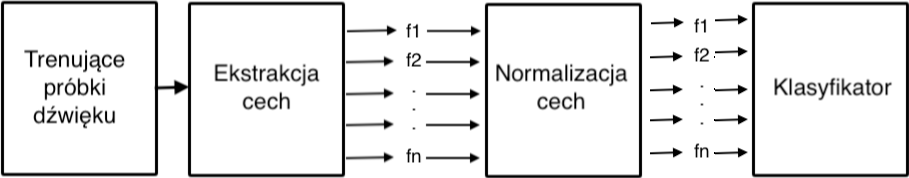
\includegraphics[scale=0.40]{trenowanie.png}
\label{ser_tren}
\end{figure}

\begin{figure}[!htb]
\hspace*{-6cm}  
	\caption{Process testowania systemu do rozpoznawania emocji z~głosu}
	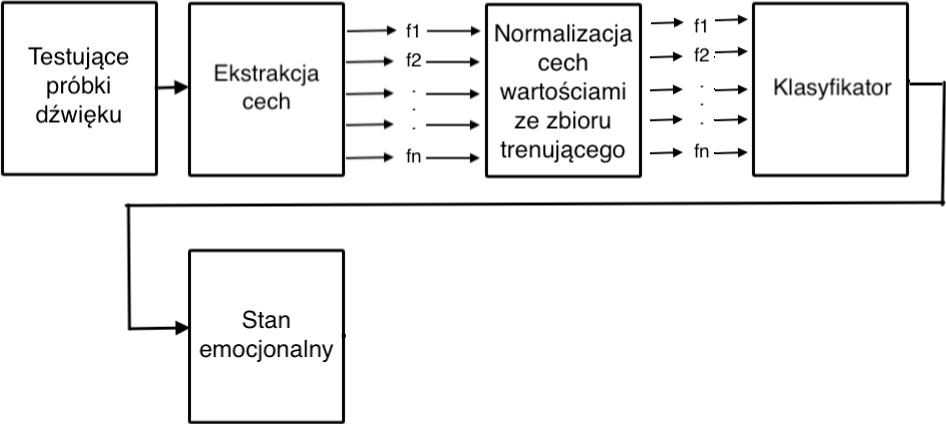
\includegraphics[scale=0.35]{testowanie.png}
\label{ser_test}
\end{figure}

\section{Dźwięk, podstawowe definicje}
Formalnie fala dźwiękowa to rozchodzące się w ośrodku zaburzenie, któremu towarzyszą drgania cząsteczek ośrodka i~która powoduje wrażenie słuchowe~\cite{Akustyka}. Fale mają pewne fundamentalne cechy jak:
\begin{enumerate}
\item Długość fali -- odległość pomiędzy początkiem a~końcem jednego pełnego cyklu.
\item Amplituda -- poziom wychylenia z~położenia równowagi. Amplituda fali akustycznej mierzona jest na 2 sposoby:
	\begin{itemize}
	\item maksymalne wychylenie -- maksymalny pozytywny lub negatywny poziom sygnału,
	\item średnia kwadratowa (RMS) -- która mierzy bardziej znaczący średni poziom sygnału.
	\end{itemize}
\item Częstotliwość -- czyli liczba pełnych drgań (cykli), jakie wykona fala w~ciągu jednej jednostki czasu (np. sekundy). Jej jednostką jest herc(Hz).
\end{enumerate}

Drganie fałd głosowych podczas wydechu powoduje wibracje, tworząc fale dźwiękowe. Następnie na skutek różnych procesów, takich jak ruchy języka, podniebienia, szczęk nabierają one specyficznych właściwości, tworząc wrażenie słuchowe nazywane głosem. Podstawowe cechy głosu to: barwa głosu, jego wysokość, oraz natężenie.

Barwa głosu zależy od ilości oraz zachowania tonów w dźwięku. To właśnie dzięki niej jesteśmy w~stanie odróżniać głosy poszczególnych osób. Właściwość ta jest mocno uzależniona od budowy gardła, krtani, fałd głosowych. 

Wysokość głosu zależy od częstotliwości fali, a dokładniej od częstotliwości tonu podstawowego. Ton to fala harmoniczna (sinuosidalna). Niższa częstotliwość tego tonu oznacza większą długość fali, a~co za tym idzie niższą wysokość. Natomiast, wraz ze wzrostem częstotliwości długość fali maleje, zmniejszając wysokość głosu. Wysokość podobnie jak częstotliwość podaje się w hercach. Ton głosu, pomimo że będzie miał taką samą wartość Hz, może być głośniejszy lub cichszy w zależności od swojej amplitudy. 

Natężenie dźwięku jest miarą energii fali dźwiękowej i~zależy od jej amplitudy.

\section{Dobór cech dźwięku}
Jak już zostało wspomniane, w projekcie w~celu rozpoznawania emocji z głosu, zdecydowano się użyć cech związanych z~wysokością głosu oraz natężeniem. Na rysunku~\ref{wyk_emo} znajdują się wykresy tych cech dla czterech emocji na których skupia się praca.

\begin{figure}[!h]
\caption{Przykładowy rozkład zmian wartości tonu podstawowego oraz natężenia w czasie}
	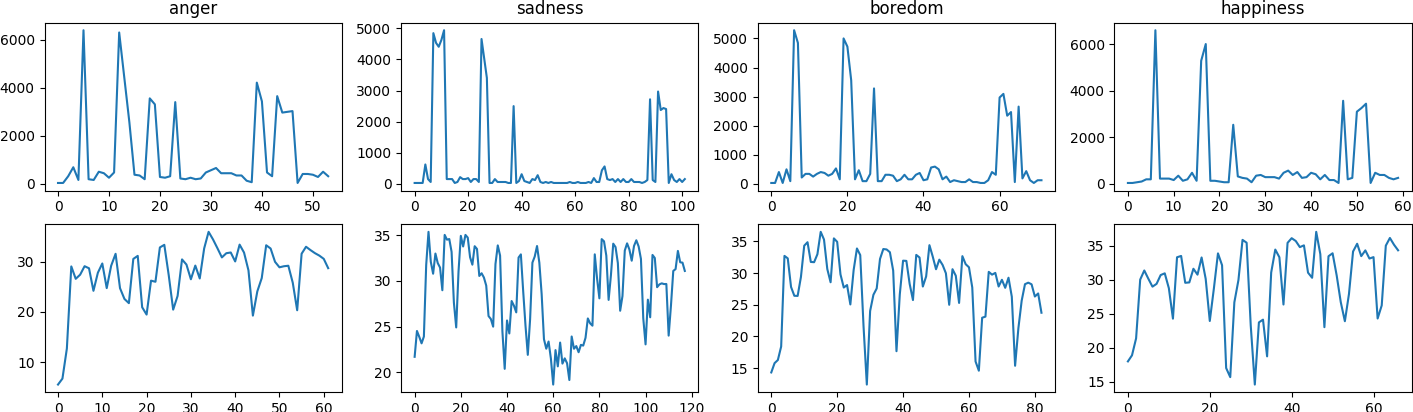
\includegraphics[scale=0.3]{b01.png}
\label{wyk_emo}
\end{figure}
	
W pierwszym wierszu dla każdej emocji widzimy rozkład tonu podstawowego w czasie, natomiast w drugim wierszu rozkład natężenia. Możemy z niego wywnioskować podstawowe zależności pomiędzy poszczególnymi emocjami. Na przykład: wysoki ton głosu i~wysoka energia są charakterystyczne  przy okazywaniu złości, natomiast również wysoki ton i~troszkę niższa energia są charakterystyczne dla szczęścia. Smutek cechuje się bardzo niskim tonem głosu i~dużą dynamiką energii, natomiast znudzenie trochę wyższym tonem głosu niż smutek, ale niższym niż dwie pozostałe emocje oraz trochę stabilniejszym poziomem energii. 

Na podstawie tych danych, informacji zaczerpniętych z~pracy~\cite{Akustyka} i~internetowego kursu~\cite{Waveform} zostało wybrane dwanaście cech, które mogłyby reprezentować stany emocjonalne.
Są to: 
\begin{enumerate}
\item różnica między maksymalna a minimalną wartością tonu podstawowego,
\item maksymalna wartość tonu podstawowego,
\item minimalna wartość tonu podstawowego,
\item średnia wartość tonu podstawowego,
\item dynamika tonu podstawowego,
\item procent tonów opadających,
\item procent tonów wzrastających,
\item relatywne standardowe odchylenie wartości tonu podstawowego,
\item relatywne standardowe odchylenie wartości średniej kwadratowej natężenia,
\item gęstość przejść przez zero,
\item średnia kwadratowa natężenia,
\item największa wartość natężenia.
\end{enumerate}

W~celu dokładniejszego doboru parametrów dźwięku skorzystano z~algorytmu ExtraTreeClassifier z~jednej z bibliotek języka Python: sklearn~\cite{sklearn}. Algorytm oblicza stopień ważności każdej z~cech. Wynik algorytmu przedstawia tabela~\ref{TWaznosc_cech}.

\begin{table}[H]
\caption{Tabela reprezentująca stopień ważności wybranych cech głosu}
\begin{tabular}{ l | r }
\label{TWaznosc_cech}
Różnica między maksymalną a minimalną wartością tonu podstawowego & 0.080200 \\
Maksymalna wartość tonu podstawowego & 0.103055 \\
Minimalna wartość tonu podstawowego & 0.098071 \\
Średnia wartość tonu podstawowego & 0.112797 \\
Dynamika tonu podstawowego & 0.020013 \\
Procent tonów opadających & 0.052253 \\
Procent tonów wzrastających & 0.047792 \\
Relatywne standardowe odchylenie wartości tonu podstawowego & 0.089292 \\
Relatywne standardowe odchylenie wartości średniej kwadratowej natężenia & 0.100254 \\
Gęstość przejść przez zero & 0.099278 \\
Średnia kwadratowa natężenia & 0.102582 \\
Największa wartość natężenia & 0.094414 \\
\end{tabular}
\end{table}

Na podstawie uzyskanych wyników zdecydowano się zrezygnować z~cechy nazwanej ,,dynamika tonu podstawowego". Ostatecznie do rozpoznawania emocji użyto pozostałych jedenastu cech.

\section{Ekstrakcja cech}

Ekstrakcja cech polega na analizie sygnału dźwiękowego i~wydobyciu z niego potrzebnych wartości. W projekcie, aby wydobyć odpowiednie cechy z sygnału dźwiękowego, co 0.125 sekundy brana jest próbka dźwięku o~długości 0.25 sekundy. Z~próbek o~tej długości wyliczane są odpowiednie cechy. Sygnał odczytywany z~pliku jest sygnałem w domenie czasu. Z takiego sygnału możemy odczytać wszystkie wartości związane z~energią, czyli:
\begin{itemize}
\item relatywne standardowe odchylenie wartości średniej kwadratowej natężenia,
\item gęstość przejść przez zero,
\item średnia kwadratowa natężenia, 
\item największa wartość natężenia.
\end{itemize}

Aby wydobyć cechy związane z~częstotliwością, należy sygnał w domenie czasu przekształcić na sygnał w~domenie częstotliwości. Operacją, która na to pozwala, jest transformacja Fouriera. W~projekcie wykorzystano algorytm szybkiej transformaty Fouriera dla rzeczywistych danych wejściowych: rfft, znajdujący się w bibliotece języka Python: numpy.fft. Z sygnału w domenie częstotliwości wydobyto częstotliwość podstawową i~na jej podstawie wyliczono pozostałe cechy.

\section{Normalizacja}

Obliczone cechy mają różną wartość. Maksymalna wartość cech obliczanych w~procentach to sto, podczas gdy maksymalna wartość częstotliwości jest dużo wyższa. Z~tego względu, podczas liczenia podobieństwa wektorów cechy z~większą rangą będą uważane jako bardziej istotne. Aby temu zapobiec, przeprowadza się normalizację wektorową. W wyniku tej operacji, wartości cech są z przedziału $\langle0,1\rangle$. Dzięki temu wpływ wszystkich cech na wynik jest taki sam. Normalizacja przebiega według następującego wzoru:

$a_i$\textprime = $\frac{a_i - min(a_i)}{max(a_i) - min(a_i)}$

\section{Klasyfikacja}
Znormalizowany wektor cech podajemy jako argumenty do klasyfikatora. Jeżeli wektor był wektorem trenującym, algorytm trenuje klasyfikator. Natomiast jeżeli wektor był wektorem testującym, to zwraca stan emocjonalny reprezentujący podany wektor cech.

\chapter{K najbliższych sąsiadów}
\section{Opis algorytmu}
K najbliższych sąsiadów (KNN) jest algorytmem często wykorzystywanym w~informatyce do klasyfikacji lub przewidywania wartości zmiennej losowej.  

W~pracy posłużono się algorytmem KNN opisanym w~podręczniku do statystyki stworzonym przez firmę StatSoft~\cite{KNN_Wstep}.
Algorytm w~trakcie trenowania nie przeprowadza żadnych obliczeń. Jedynie zapamiętuje zbiór wektorów trenujących $T$ w~postaci [$X_i$, $Y_i$], gdzie $X_i$~oznacza $i$-tą~obserwację, natomiast $Y_i$ przewidywaną zmienną $i$-tej obserwacji.

Podczas testowania podana jest obserwacja $O$. Celem algorytmu jest prognoza przewidywanej wartości tej obserwacji. W~tym celu algorytm:
\begin{enumerate}
\item oblicza odległość pomiędzy $O$~a~każdą z~obserwacji ze zbioru trenującego;
\item tworzy zbiór $O\textprime$, w~którego skład wchodzi $k$~najbliżej położonych od niego obserwacji ze zbioru trenującego;
\item przeprowadza głosowanie wśród elementów ze zbioru $O\textprime$~i~obserwacji $O$~przypisuje element, który wystąpił największą ilość razy.
\end{enumerate}

\section{Implementacja}
W części trenującej program tworzy moduł KNN i~podaje mu zbiór wektorów w postaci [wektor cech, emocja jaką reprezentuje]. Moduł KNN normalizuje wektory ze zbioru, zapamiętuje je oraz parametry użyte do normalizacji.

W części testującej program podaje modułowi KNN zbiór wektorów cech $V$~wypowiedzi. Algorytm KNN najpierw dla każdego wektora $w \in V$ normalizuje $w$~wartościami użytymi do normalizacji zbioru trenującego, a~następnie przeprowadza algorytm testowania opisany na początku tego rozdziału. Jako emocję reprezentującą wypowiedź algorytm zwraca emocję, która została najczęsciej przypisana wektorom ze zbioru $V$. Jeżeli więcej niż jedna emocja wystąpiła najczęściej, zwracana jest losowa z~nich.  

\chapter{Ukryte Modele Markowa}
\section{Opis modelu}
Ukryte modele Markowa (HMM) to narzędzie służące do statystycznej analizy sekwencji zdarzeń. Aby zrozumieć ten model, należy zacząć od 
definicji łańcucha Markowa.

Łańcuch Markowa jest modelem składającym się ze zbioru stanów $S$~oraz macierzy $M$, zawierającej prawdopodobieństwa przejść pomiędzy stanami. Opisuje układ, który w danym momencie czasu może znajdować się tylko w jednym ze swoich stanów, a~w~następnym przejść do innego lub pozostać w~swoim z~prawdopodobieństwem zapisanym w macierzy $M$. Cechą charakterystyczną dla łańcucha Markowa jest to, że zachowuje on własność Markowa, która mówi, że w czasie $t+1$~prawdopodobieństwo bycia w stanie $j$~zależy jedynie od stanu w~jakim układ znajdował się w~czasie $t$.

Ukryty model Markowa jest modelem zawierającym:
\begin{itemize}
\item stany, które tworzą łańcuch Markowa
\item zbiór możliwych obserwacji
\item macierz prawdopodobieństw przejść pomiędzy stanami $M$~($M_{ij}$~oznacza prawdopodobieństwo przejścia ze stanu $i$~do stanu $j$)
\item macierz emisji $E$~($E_{ij}$~oznacza prawdopodobieństwo emisji obserwacji $j$~w~stanie $i$)
\end{itemize}

Ukryte Modele Markowa zakładają, że stany tworzące łańcuch Markowa są ukryte. Widoczna jest tylko obserwacja jaką stan zwróci. Na tej podstawie i~mając dane z tablicy emisji oraz przejść, HMM jest w stanie obliczyć prawdopodobną sekwencję stanów, która wyrzuciła dany wektor obserwacji oraz prawdopodobieństwo wygenerowania obserwacji w modelu.

W projekcie wykorzystano liniowy model HMM~\cite[Chapter~8.1]{HMM_pattern}. Charakteryzuje on się tym, że w czasie $t$, ze stanu $s_{i}$~możemy przejść do stanu $s_{i+1}$~lub pozostać w stanie $s_{i}$, z pewnym prawdopodobieństwem. Prawdopodobieństwo przejścia do pozostałych stanów jest zerowe. Do trenowania ukrytych modeli Markowa wykorzystano algorytm Bauma-Welcha, natomiast w~celu obliczenia prawdopodobieństwa wygenerowania obserwacji przez model wykorzystano algorytm prefiksowy. Definicje i~dokładny opis algorytmów można znaleźć w pracy ,,Wstęp do ukrytych modeli Markowa i~metody Bauma–Welcha"~\cite{HMM_Wstep}.

\section{Implementacja}
W pierwszej fazie program tworzy zbiór wszystkich możliwych obserwacji. W~tym celu, z~każdego pliku w~zbiorze trenującym pobiera wektory cech. Kolejnym etapem jest normalizacja stworzonego zbioru wektorów. W~celu zmniejszenia liczby obserwacji i~uśrednienia ich program używa algorytmu k-średnich, o~nazwie KMeans z~biblioteki sklearn~\cite{sklearn}. Algorytm tworzy podaną ilość możliwych obserwacji.

W~części trenującej program dla każdej emocji i~każdego pliku trenującego reprezentującego tę emocję tworzy zbiór sześciu wektorów cech, będących sekwencją 1,5-sekundowej wypowiedzi. Każdy wektor cech reprezentuje 0.25 sekundy wypowiedzi. Następnie wektory zostają znormalizowane $i$ każdy z~nich zostaje zamieniony na najbliższą jej obserwację ze zbioru obserwacji. Dzięki temu algorytm jest w~stanie ją rozpoznać. Następnie dla każdej emocji tworzy oddzielmy model HMM i~trenuje go zbiorem sekwencji odpowiadających emocji, jaką reprezentuje model.

\begin{figure}[!ht]
\hspace*{-5cm}  
	\caption{Process trenowania modelu HMM do rozpoznawania emocji z głosu}
	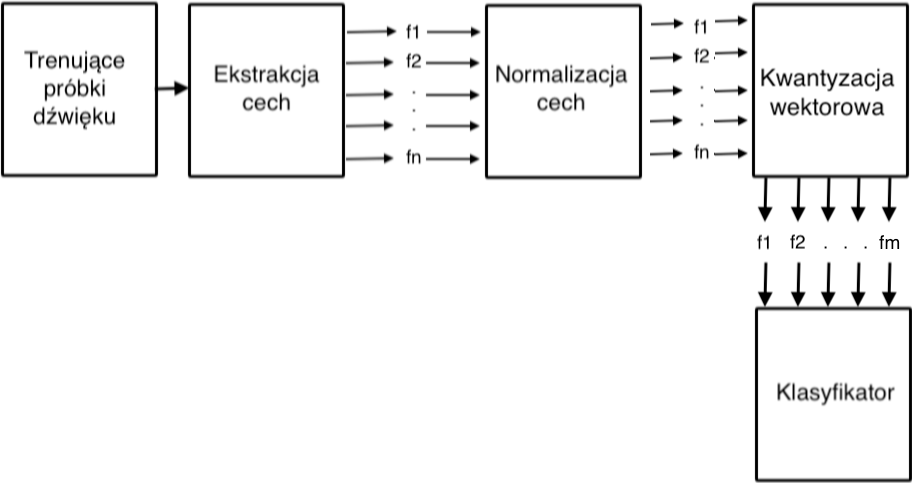
\includegraphics[scale=0.35]{hmm_train.png}
\end{figure}

Podczas testowania z~pliku będącego wypowiedzią, algorytm oblicza zbiór obserwacji $O$. Każdy z~elementów obserwacji reprezentuje zbiór 6 wektorów cech będących sekwencją 1,5-sekundowej wypowiedzi. Kolejnym krokiem jest normalizacja każdej obserwacji, wartościami, którymi był normalizowany zbiór wszystkich możliwych wartości. Każdy ze znormalizowanych wektorów cech zostaje zamieniony na najbliższy mu wektor ze zbioru obserwacji, tworząc zbiór $S$. Dzięki temu model HMM będzie je rozpoznawał. Następnie, program dla każdej obserwacji ze zbioru $S$~i~każdego modelu HMM, wylicza prawdopodobieństwo wygenerowania tej obserwacji w~tym modelu. Jako emocję, która odpowiada tej obserwacji wybiera tą, która reprezenutje model HMM, który wyliczył największe prawdopodobieństwo jej wygenerowania. Jako emocję reprezentujacą wypowiedź algorytm zwraca emocję, która po przejściu wszystkich obserwacji ze zbioru $O$~wystąpiła najcześciej. Jeżeli więcej niż jedna emocja wystąpiła najczęściej, zwracana jest losowa z~nich.

\chapter{Wyniki}
\section{Baza danych mowy emocjonalnej}
W~celu przetestowania algorytmów użyto niemieckiej bazy mowy emocjonalnej~\cite{BDemo}. Wybrano właśnie tę bazę danych, ponieważ jest ona publicznie dostępna oraz w~istniejących rozwiązaniach, testy na tej bazie danych charakteryzowały się dużą poprawnością. Ponadto baza zawiera wszystkie 4 emocje, na których skupia się ten projekt.

\section{Wyniki}
W algorytmie KNN, najlepszy wynik został wygenerowany przy liczbie stanów równej 17. Wyniki prezentuje tabela~\ref{KNN_result}.

\begin{table}[p]
\caption{Tabela przedstawiająca wyniki działania programu rozpoznajacego emocje z użyciem algorytmu k najbliższych sąsiadów}
\begin{center}
  \begin{tabular}{|c|c|c|c|c|}
    \hline
    emocja & szczęście & złość & smutek & znudzenie \\ \hline
    szczęście & 39.13\% & 60.86\% & 0\% & 0\% \\ \hline
	złość & 12,5\ & 85\% & 0\% & 2,5\% \\ \hline
	smutek & 0\% & 0\% & 95,83\% & 4,16\% \\ \hline
	znudzenie & 0\% & 7,69\% & 38,46\% & 53,85\%\\ 
	\hline
  \end{tabular}
  \label{KNN_result}
\end{center}
\end{table}

Widać z~niej, że algorytm k~najbliższych sąsiadów wykrył poprawnie 68.45\% emocji. Najlepiej radzi sobie z~emocjami, które cechują się wyrazistymi różnicami jak złość, którą cechuje wysoki ton i wysoka energia oraz smutek, który cechuje niski ton i niska energia. Natomiast gorzej radzi sobie z~emocjami, których właściwości nie są tak wyraziste. Szczęście w~39,13\% myli ze złością, która cechuje się podobnymi parametrami, natomiast znudzenie myli w~38,46\% ze smutkiem. A więc na podstawie wyników algorytmu można również stwierdzić podobieństwo sposobu wyrażania poszczególnych emocji.

System rozpoznający emocje z~głosu bazujący na ukrytych modelach Markowa został przetestowany na stanach od 200, do 700. Najlepsze wyniki pod kątem poprawności i~szybkości działania uzyskał dla 500 stanów. Tabela~\ref{HMM_result} prezentuje wyniki algorytmu: 

\begin{table}[p]
\caption{Tabela przedstawiająca wyniki działania programu rozpoznajacego emocje z użyciem algorytmu bazujacego na ukrytych modelach Markowa}
\begin{center}
  \begin{tabular}{| c | c | c | c | c |}
    \hline
    emocja & szczęście & złość & smutek & znudzenie \\ \hline
    szczęście & 39,13\% & 47,83\% & 8,70\% & 4,35\% \\ \hline
	złość & 10\% & 72,5\% & 0\% & 2,5\% \\ \hline
	smutek & 0\% & 0\% & 91,87\% & 8,33\% \\ \hline
	znudzenie & 0\% & 3,85\% & 50\% & 46,15\% \\
    \hline
  \end{tabular}
  \label{HMM_result}
\end{center}
\end{table}

Widać z~niej, że algorytm bazujący na Ukrytych Modelach Markowa wykrył poprawnie 62,41\% emocji. Podobnie jak KNN bardzo dobrze rozpoznaje emocje takie smutek czy złość. Natomiast gorzej radzi sobie z emocjami takimi jak szczęście i~znudzenie, myląc je odpowiednio ze~złością i~smutkiem.

Oba wyniki mają podobne cechy. Mylą szczęście ze złością oraz znudzenie ze smutkiem. Jak przyjrzymy się jeszcze raz wykresom z~rysunku \ref{wyk_emo}, możemy zauważyć podobieństwo wysokości i~natężenia głosu w tych emocjach. Jak widzimy na przykładzie szczęścia i~złości, szczęście ma niewiele mniejsze parametry co złość. Podobnie z~pozostałymi dwoma emocjami. W celu dokładniejszego porównania podobieństwa cech tych emocji obliczono średnią wartość tych cech z~wszystkich wypowiedzi ze zbioru trenującego. Tabela~\ref{sr_war} prezentuje uzyskane wyniki:

\begin{table}[p]
\caption{Tabela przedstawiająca średnie wartości cech dla każdej z emocji}
  \begin{tabular}{|l|c|c|c|c|}
    \hline
    cecha/emocja & złość & szczęście & smutek & znudzenie \\ \hline
    Ranga tonu głosu & 1984.25 & 1869.97 & 1172.018 & 1169.39 \\ \hline
    Maksymalny ton & 2180.92 & 2052.31 & 1238.78 & 1274.70\\ \hline
    Minimalny ton & 196.67 & 182.34 & 66.77 & 105.31 \\ \hline
    Średnia wartość tonu & 879.42 & 801.53 & 439.23 & 487.50\\ \hline
	Procent tonów opadających & 46.54 & 45.24 & 32.95 & 36.35 \\ \hline
	Procent tonów wzrastających & 44.13 & 42.20 & 31.98 & 35.16 \\ \hline
	Std odchylenie tonu podstawowego & 80.16 & 80.56 & 80.09 & 74.31 \\ \hline
	Std odchylenie natężenia & 40.84 & 36.51 & 29.27 & 29.35 \\ \hline
	Gęstość przejść przez zero & 2.04 & 1.48 & 0.76 & 0.76 \\ \hline
	Średnia kwadratowa natężenia & 29.43 & 29.69 & 30.04 & 31.29 \\ \hline
	Największa wartość natężenia & 15.08 & 14.22 & 12.25 & 12.71 \\ \hline
  \end{tabular}
  \label{sr_war}
\end{table}

Z powyższej tabeli można odczytać, że średnie wartości cech w~emocjach, które algorytmy mylą są bardzo podobne. Przez to szczęście często mylone jest ze złością, która cechuje się niewiele większymi parametrami i~nachodzi na tę emocję. Podobnie jest w przypadku znudzenia i~smutku. 

Pomimo podobieństw widać, że algorytmy całkiem dobrze poradziły sobie z zadaniem. Cechy, które w projekcie użyto nie wystarczą do dokładnego rozpoznawania emocji z~głosu, ale nadają sie do rozpoznawania podstawowych emocji, zmian stanu z pobudzonego na spokojny i~wiele innych. Wynik działania algorytmu można poprawić dodajac dodatkowe cechy na przykład na cechy związane z: jakością głosu (prędkość mówienia, płynność) lub cechy spektralne MFCC, LFPC. 

\chapter{Wnioski i podsumowanie}
Algorytm k najbliższych sąsiadów poradził sobie lepiej z~tym problemem. Jednakże różnica jest niewielka. Poprawność wyników, jakie zwróciły oba algorytmy, wynosi ponad 60\%. Jednak algorytm KNN jest prostszy do zaimplementowania oraz czas działania tego algorytmu jest szybszy. Także biorąc pod uwagę również te cechy, spisuje się o~wiele lepiej.

Warto jednak zwrócić uwagę, że istnieje dużo różnych możliwości implementacji ukrytych modeli Markowa, oraz sposobów trenowania go. W projekcie zdecydowano się użyć modelu liniowego oraz do trenowania, algorytmu Bauma-Welcha. Inny model może zwrócić zupełnie inne wyniki.

Projekt inżynierski opracowany w~tej pracy ma za zadanie rozpoznawać cztery podstawowej emocje: szczęście, złość, smutek oraz znudzenie. Do swojego działania wykorzystuje jeden z~dwóch algorytmów: k najbliższych sąsiadów lub algorytmu bazującego na ukrytych modelach Markowa, w~zależności od wyboru użytkownika. Ponadto do projektu dodano dodatkową opcję, która pozwala śledzić przebieg częstotliwości i~natężenia w~czasie w~plikach .wav. Praca została wykonana w pełnym zakresie i~zgodnie z~założonym celem. Wyniki pracy zostały zaprezentowane i~opisane w~pracy. Do projektu jest załączona dokumentacja w~postaci html i~pdf, która zawiera opis funkcji programu.

Projekt można rozwinąć. Możliwe usprawnienia:
\begin{itemize}
\item dodanie kolejnych cech dźwięku w celu przetestowania wpływu tych właściwości na poprawne rozpoznawanie emocji,
\item dodanie większej liczby emocji,
\item implementacja innych algorytmów w celu przetestowania ich działania w tym problemie.
\end{itemize}

\listoffigures
\listoftables
\nocite{*}
\addcontentsline{toc}{chapter}{Bibliografia}
\printbibliography
\end{document}
